\documentclass[11pt,a4paper]{article}

% --- Paquetes de Estilo y Formato ---
\usepackage[utf8]{inputenc}
\usepackage[spanish,es-tabla]{babel}
\usepackage[T1]{fontenc}
\usepackage{geometry}
\geometry{top=3cm, bottom=3cm, left=3cm, right=2.5cm}
\usepackage{tabularx}
\usepackage{titlesec}
\usepackage{fancyhdr}
\usepackage{lastpage}
\usepackage{hyperref}
\usepackage{enumitem}
\usepackage{graphicx}
\usepackage{tikz}
\usepackage{float}
\usepackage[table, xcdraw]{xcolor}

% --- Definición de Colores Corporativos ArthroDesign ---
\definecolor{ArthroNavy}{HTML}{0F172A}
\definecolor{ArthroTeal}{HTML}{0D9488}
\definecolor{ArthroGray}{HTML}{64748B}

% --- Configuración de Párrafo ---
\setlength{\parskip}{0.5em}
\setlength{\parindent}{1.5em}

% --- Estilo de Títulos con Identidad Corporativa ---
\titleformat{\section}
  {\color{ArthroNavy}\Large\bfseries}
  {\thesection.}
  {0.5em}
  {}
  [{\color{ArthroTeal}\titlerule[1.5pt]}]

\titleformat{\subsection}
  {\color{ArthroNavy}\large\bfseries}
  {\thesubsection.}
  {0.5em}
  {}
  [{\color{ArthroTeal}\titlerule[1pt]}]

\titleformat{\subsubsection}
  {\color{ArthroNavy}\large\bfseries}
  {\thesubsubsection.}
  {0.5em}
  {}

% --- Viñetas en color Turquesa ---
\renewcommand{\labelitemi}{\color{ArthroTeal}\textbullet}
\renewcommand{\labelitemii}{\color{ArthroTeal}\circ}

% --- Configuración de Enlaces ---
\hypersetup{colorlinks=true, linkcolor=ArthroNavy, urlcolor=ArthroTeal}

% --- CONFIGURACIÓN DE ENCABEZADO Y PIE CORPORATIVO (Anexo VIII) ---
\pagestyle{fancy}
\fancyhf{}

% Línea superior de color turquesa (Grosor 2pt)
\renewcommand{\headrule}{\hbox to\headwidth{\color{ArthroTeal}\leaders\hrule height 2pt\hfill}}

% Información de Encabezado
\fancyhead[L]{\small \textbf{\color{ArthroNavy}Adaptador ergonómico - PR-PIB-GIS26-09}}
\fancyhead[R]{\small \textbf{\color{ArthroNavy}Anexo VII: Ilustraciones}}

% Información de Pie de Página
\fancyfoot[L]{\small \color{ArthroGray}ArthroDesign Solutions S.L.}
\fancyfoot[C]{\small \color{ArthroGray}\today}
\fancyfoot[R]{\small \textbf{\color{ArthroNavy}Pág. \thepage \ de \pageref{LastPage}}}

\setlength{\headheight}{15pt}
\renewcommand{\footrulewidth}{0.4pt}

\begin{document}

% ======================================================
% PÁGINA 1: PORTADA TÉCNICA (BLOQUE SÓLIDO)
% ======================================================
\begin{titlepage}
    
    % --- LOGO CORPORATIVO (Alineado a la derecha) ---
    \begin{flushright}
        \vspace*{-2cm}
        
\includegraphics[width=7.5cm]{logo_definitivo.png}
    \end{flushright}

    \vspace{-0.5cm}

    \begin{flushleft}
        % --- ETIQUETA DEL VOLUMEN ---
        {\color{ArthroGray}\Large \textbf{DOCUMENTO Nº 3: ANEXOS}} \\[0.5cm]
        
        % --- BLOQUE SÓLIDO DE IDENTIFICACIÓN DEL ANEXO ---
        \noindent\colorbox{ArthroNavy}{%
            \parbox{\dimexpr\textwidth-2\fboxsep\relax}{%
                \vspace{0.5cm}
                \centering
                \hspace{0.2cm}{\color{white}\fontsize{42pt}{48pt}\selectfont\textbf{ANEXO VII}}
                \vspace{0.5cm}
            }%
        } \\[0.8cm]
        
        % --- TÍTULO DEL ANEXO ---
        \centering
        {\color{ArthroTeal}\Huge\bfseries ILUSTRACIONES} \\[0.4cm]
        {\color{ArthroGray}\rule{\textwidth}{1.5pt}} \\
        
        \vspace{0.6cm}

        % --- INFORMACIÓN DEL PROYECTO MAESTRO ---
        \centering
        {\color{ArthroNavy}\small\textbf{TÍTULO DEL PROYECTO:}} \\[0.3cm]
        {\huge\bfseries Diseño de un adaptador ergonómico universal para la optimización de la pulsación manual en inhaladores de dosis medida (MDI)} \\
        
        \vspace{1cm}

        % --- BLOQUE DE IDENTIFICACIÓN TÉCNICA ---
                \centering
                {\color{ArthroGray}\small\textbf{CÓDIGO DE IDENTIFICACIÓN:}} \\ {\large\texttt{PR-PIB-GIS26-09}} \\
                \vspace{0.5cm}
                {\color{ArthroGray}\small\textbf{PROMOTOR Y EMPRESA DESARROLLADORA:}} \\ {\large ArthroDesign Solutions S.L.} \\{Calle Severo Ochoa, Nº 12, 29590 Málaga, España}\\
        {NIF: B12345678} \\
        \href{mailto:contacto@arthrodesign.com}{contacto@arthrodesign.com} \\
  

        \vspace{1cm}

        % --- BLOQUE DE PROYECTISTAS AUTORES ---
        {\color{ArthroNavy}\small\textbf{PROYECTISTAS (Equipo de ArthroDesign Solutions S.L.):}} \\[0.3cm]
        \small
        \renewcommand{\arraystretch}{1.4}
        \begin{tabular}{@{}l l}
            \textbf{D. Sergio Carmona Muñoz} & Colegiado Nº 06424 (DNI: 26291930D) \\
            \textbf{D. Juan Gabriel Navarro Valdivielso} & Colegiado Nº 06425 (DNI: 77666662D) \\
            \textbf{D. Antonio Sánchez Doña} & Colegiado Nº 06423 (DNI: 79380534J) \\
            \textbf{D. Iván de la Torre Segato} & Colegiado Nº 06421 (DNI: 79383630G) \\
        \end{tabular}

        \vfill

        % --- PIE DE PORTADA ---
        {\color{ArthroTeal}\rule{\linewidth}{1pt}} \\[0.3cm]
        \small\color{ArthroGray}  ArthroDesign Solutions S.L. \quad | \quad \today
    \end{flushleft}
\end{titlepage}

% AÑADE ESTA LÍNEA AQUÍ PARA QUE LA SIGUIENTE PÁGINA SEA LA 2:
\setcounter{page}{2}

% ======================================================
% HOJA EN BLANCO CON MARCA DE AGUA
% ======================================================
\newpage
\pagestyle{fancy}

\begin{tikzpicture}[remember picture, overlay]
    \node[opacity=0.1] at (current page.center) {
\includegraphics[width=12cm]{logo_definitivo.png}};
\end{tikzpicture}

% Empujamos el texto hacia la parte inferior del folio
\vspace*{8.5cm} 
\begin{center}
    \textit{Esta hoja ha sido dejada deliberadamente en blanco.}
\end{center}
\vfill
\newpage

% ======================================================
% PÁGINA: ÍNDICE AUTOMÁTICO (CON ENCABEZADO)
% ======================================================
\markboth{Índice}{Índice}
\tableofcontents
\thispagestyle{fancy} % Fuerza el estilo fancy en esta página
\newpage

% ======================================================
% PÁGINA: ÍNDICE DE FIGURAS
% ======================================================
\markboth{Índice de figuras}{Índice de figuras}
\listoffigures
\thispagestyle{fancy}
\newpage




% ======================================================
% DESARROLLO DEL PRODUCTO EN CAD (NUEVO CONTENIDO)
% ======================================================
\newpage
\section{DISEÑO DE DETALLE EN CAD}


\subsection{Fase 1: Modelado del inhalador (MDI)}


\begin{figure}[H]
    \centering
   
   
     
\includegraphics[width=0.8\textwidth]{ANEXOS/CAD_Inhalador.png}
    \caption{Modelo CAD del Inhalador de Dosis Medida (MDI) usado como referencia.}
    \label{fig:cad_inhalador}
\end{figure}


\subsection{Fase 2: Diseño de la base}


\begin{figure}[H]
    \centering
   
    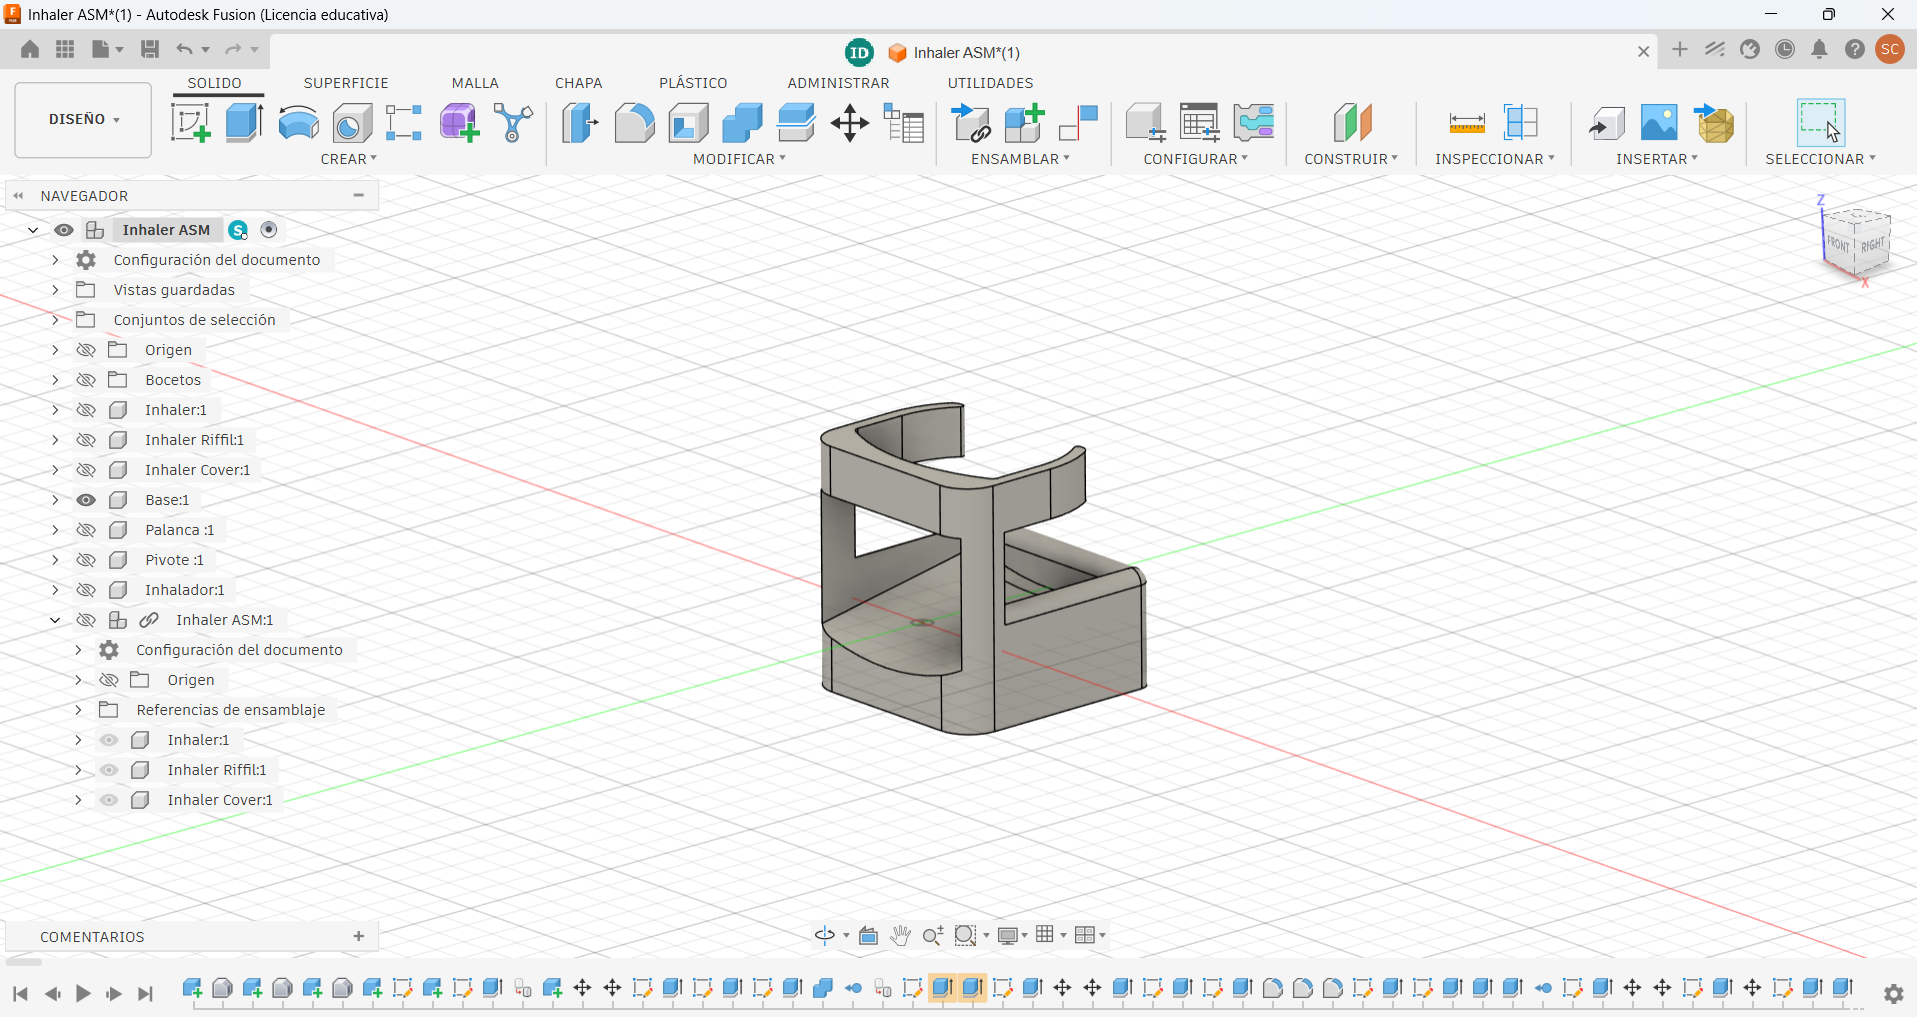
\includegraphics[width=0.8\textwidth]{CAD_Base.png}
    \caption{Diseño CAD de la Base del adaptador.}
    \label{fig:cad_base}
\end{figure}

\newpage
\subsection{Fase 3: Desarrollo del pivote}

\begin{figure}[H]
    \centering
   
    
\includegraphics[width=0.8\textwidth]{CAD_Pivote.png}
    \caption{Modelo CAD del Pivote articulado.}
    \label{fig:cad_pivote}
\end{figure}

\subsection{Fase 4: Diseño de la palanca}


\begin{figure}[H]
    \centering
   
     
\includegraphics[width=0.8\textwidth]{CAD_Palanca.png}
    \caption{Diseño CAD de la Palanca de actuación.}
    \label{fig:cad_palanca}
\end{figure}
\newpage
\subsection{Fase 5: Ensamblaje completo}


\begin{figure}[H]
    \centering
   
     
\includegraphics[width=0.8\textwidth]{ANEXOS/CAD_Ensamblaje.png}
    \caption{Ensamblaje completo de todos los componentes}
    \label{fig:cad_palanca}
\end{figure}


% ======================================================
% BLOQUE DE FIRMAS
% ======================================================
\vspace{2cm}
\noindent\begin{minipage}{\textwidth}
    \begin{flushright}
        En Málaga, a \today
    \end{flushright}
    \vspace{2cm}

    \noindent
    \begin{minipage}[t]{0.45\textwidth}
        \centering
        \rule{6cm}{0.6pt} \\
        \textbf{Fdo. D. Sergio Carmona Muñoz} \\
        Colegiado Nº 06424 \\
        DNI: 26291930D
    \end{minipage}
    \hfill
    \begin{minipage}[t]{0.45\textwidth}
        \centering
        \rule{6cm}{0.6pt} \\
        \textbf{Fdo. D. Juan Gabriel Navarro Valdivielso} \\
        Colegiado Nº 06425 \\
        DNI: 77666662D
    \end{minipage}

    \vspace{2cm}

    \noindent
    \begin{minipage}[t]{0.45\textwidth}
        \centering
        \rule{6cm}{0.6pt} \\
        \textbf{Fdo. D. Antonio Sánchez Doña} \\
        Colegiado Nº 06423 \\
        DNI: 79380534J
    \end{minipage}
    \hfill
    \begin{minipage}[t]{0.45\textwidth}
        \centering
        \rule{6cm}{0.6pt} \\
        \textbf{Fdo. D. Iván de la Torre Segato} \\
        Colegiado Nº 06421 \\
        DNI: 79383630G
    \end{minipage}
\end{minipage}
\vspace{1cm}

% ======================================================
% HOJA EN BLANCO CON MARCA DE AGUA
% ======================================================
\newpage
\pagestyle{fancy}

\begin{tikzpicture}[remember picture, overlay]
    \node[opacity=0.1] at (current page.center) {
\includegraphics[width=12cm]{logo_definitivo.png}};
\end{tikzpicture}

% Empujamos el texto hacia la parte inferior del folio
\vspace*{8.5cm} 
\begin{center}
    \textit{Esta hoja ha sido dejada deliberadamente en blanco.}
\end{center}
\vfill

\end{document}